% $Id: gui_data.tex 395 2011-11-17 22:34:59Z cphillip $
%
% Written by Maria Joao Rosa
%_______________________________________________

\chapter{Data \& Design}
\label{chap:DataDesign}
\minitoc

\section{Introduction}

The first step in a statistical analysis of neuroimaging data,  whether it's in a pattern recognition or general linear model (GLM) framework, usually entails providing to the analysis software all the information regarding the data and experimental design. PRoNTo is no exception. After preprocessing the data (if required), the analysis in PRoNTo starts with the `Data and Design' module. It is important to note that PRoNTo does not perform any spatial or temporal pre-processing, and if not performed with another software, pattern recognition might be affected by misalignment and noise in the data. 

In the `Data and design' module the user can enter the image/scan files, experimental conditions (TR, durations and onsets of events), as well as other parameters, covariates and regression values. PRoNTo supports multi-modality datasets and therefore it allows the user to enter more than one data modality, such fMRI, MRI, PET and ASL, per analysis. This module is therefore essential for the rest of the framework and stores all the information that is needed from the data to be used by the rest of the software modules, such as feature set preparation, model specification and estimation. 

Below is a summary of what the `Data and Design' module does. The Methods section discusses how the module is organised and what its main output is. It also mentions a few issues that need to be taken into consideration when entering the information and how they affect subsequent steps. This chapter then presents the graphical user interface (GUI) that is used to enter the data and design information and how it is used. Finally, the chapter finishes by mentioning the corresponding `Data and Design' {\tt matlabbatch} module, and particular issues that do not apply to the GUI.

\section{Methods}

\subsection{Data and design input}

PRoNTo provides two types of interfaces for entering the data and design information, a PRoNTo-specific graphical user interface (GUI) and the  {\tt matlabbatch} system that is also currently used by SPM. These two interfaces are also available for the other modules, as discussed in the Introduction chapter.

The information that needs to be entered is almost exactly the same for both the GUI and batch (the small differences are explained below in the  {\tt matlabbatch} section) and, more importantly, the output is exactly the same. Therefore it is up to the user to decide which system is best suited for his/her analyses. For instance, the GUI can be used as a first approach to the toolbox and by users not familiar with SPM, whilst the batch can be used by more advanced or SPM users, who know how to take advantage of the batch system to optimise their analyses.

As mentioned, PRoNTo supports multi-modality analyses. Therefore the data and design module is prepared to receive as input the following types of data: fMRI, sMRI, PET and beta images (created from a previous GLM analysis). Other types of data can also be entered at the user's risk, as long as they comprise nifti files.

Regardless of which interface the user chooses to enter the data and design (GUI or batch), the organisation is very similar and starts (after choosing the directory to save {\tt PRT.mat}) with the definition of Groups. In neuroimaging datasets, it is common to have a few subjects with a lot of images/scans per subject, such as the time-series in fMRI. However, the opposite is also common: lots of subjects with one image per subject, such as encountered in PET or MRI studies. Therefore, for each group, PRoNTo provides two ways of entering the rest of the information, i.e. subjects, modalities and design, which are referred to as the `select by subject' or `select by scans' option, respectively (as is shown below). If one chooses to enter the data by `scans', PRoNTo allows the user to enter, for each modality, all subjects (one image/scan per subject) at once, which is a lot quicker than entering each subject at a time. It is important to note that when using \textit{Regression} models this is the only way of inputing the data. As explained below, only the `select by scans' option allows the users to enter regression values (one value per subject/image). This option however is not appropriate for modalities which have an experimental design and more than one image per subject, such as fMRI. For these datasets the user should choose the `subjects' option. For each subject one can specify the modalities, experimental conditions and enter more than one image/scan. Both options are valid and produce exactly the same output structure (if used with the same dataset). 

\subsection{Data and design output}

The output of the `Data and Design' module is the PRT structure (as discussed in the Introduction). This structure contains subfields with all the information that is needed from the data for the subsequent analysis steps and it is saved in a `PRT.mat' file. For advanced users the fields of this structure can be edited directly and saved, therefore bypassing the need to use the GUI or  {\tt matlabbatch} to create the PRT. However, this structure is the core of PRoNTo and should be carefully created because it affects everything else.

\subsection{Review}

The `Data and Design' module also allows the user to review the information that has been entered (through the GUI, batch or manually). The main aim of the `Review' function is to check if the data and design has been correctly specified. It can also be used to inspect if the design is appropriate for subsequent analysis. For example, the review window shows the number of subjects in each group, and for modalities with experimental design, it can be used to show and alter the number of used and unused scans (see below). 

\subsection{HRF correction}

For datasets such as fMRI, there is a very important issue that needs to be carefully addressed when specifying the data and design. As is well known, the hemodynamic response function (HRF) is a delayed and dispersed version of the underlying neuronal response to an experimental event (Figure \ref{Fig2.1}). This means that, depending on the TR, the effect of the HRF can be felt over multiple scans, and therefore the acquired scans are not independent and might contain information from both past and present events. This can confound subsequent analyses and needs to be accounted for. For instance, in SPM, the stimulus time-series are convolved with a canonical HRF. Although convenient in the GLM framework, the convolution approach is not appropriate in the pattern recognition context. Therefore, the solution used in PRoNTo is to discard all overlapping scans. This is done as follows: PRoNTo allows the user to control a delay (time it takes for the hemodynamic response to peak after the stimulus) and overlap (width of the response) parameter that determine the shape of the HRF. As can be seen in Figure \ref{Fig2.1}, the delay means that the scans corresponding to a given condition are actually shifted in time, and the overlap means that the number of independent scans, for which the signal corresponds only to a given condition, is smaller than the total number of acquired scans for each condition. Given the delay, PRoNTo finds which scans correspond to each condition and discards the last scans in the time-series for which the response has not yet peaked. It then uses the overlap to determine which consecutive scans contain information from only one condition (i.e. the response does not overlap with the response from the previous condition) and discards the ones for which there is overlap (as shown in Figure \ref{Fig2.1}, bottom right). The discarded scans are not actually deleted but are not used in further analyses.

When using the GUI, the default value for the HRF parameters is 0 seconds and can only be changed in the `Review' window (as shown below). Therefore, for fMRI, the user should review the data and design and change these parameters to a more appropriate value (e.g. 6 seconds each). In the {\tt matlabbatch}, the default value for these parameters is also 0 seconds but can be changed directly within the batch (no need to open Review window). Again, for fMRI, these values should be changed (e.g. to 6 seconds).

Importantly, if one wants to avoid discarding scans and having to correct for the shape of the HRF, as explained in the above paragraph, one should use as input the beta (coefficients) images obtained by first running a GLM analysis on the original data. The GLM analysis accounts for the HRF delay and overlap using the convolution approach. This is normally the best approach in case of rapid event-related design experiments, in which there can be a lot of overlap, i.e. the number of discarded scans can be very high.

\begin{figure}[!h]
  \begin{center}
      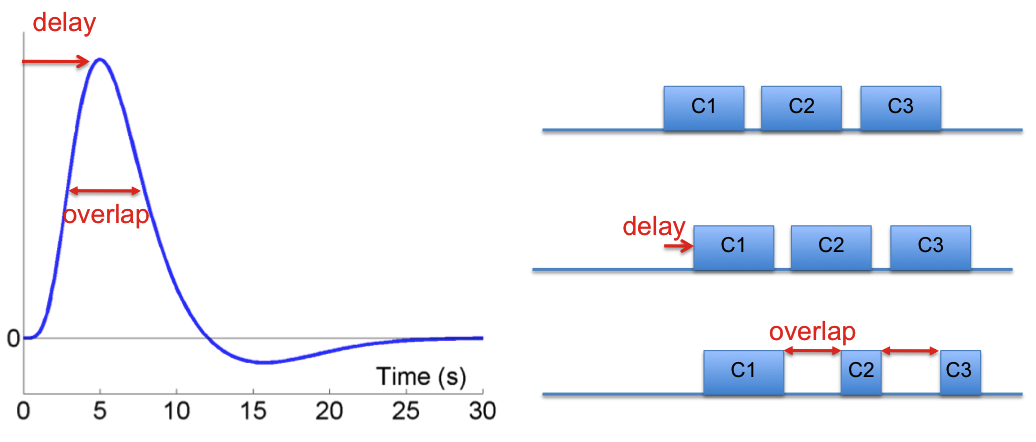
\includegraphics[height=2.2in]{images/Figure1.png}
   \caption{HRF correction. On the left is the standard HRF response. On the right is the effect of the delay and overlap on the number of independent scans (C1, C2 and C3 correspond to three different experimental conditions and the blue boxes correspond to various scans acquired during each condition). In fMRI datasets, the nature of the HRF (i.e. being a delayed and dispersed version of the neuronal response to an experimental event) might lead to less independent scans/events than the ones originally acquired. In PRoNTo, this issue is accounted for by discarding overlapping scans.}
    \label{Fig2.1}
  \end{center}
\end{figure}

The steps to specify the information relative to the data and design using both the GUI and the {\tt matlabbatch} system are described in the following sections.

\section{Graphical User interface}

The graphical user interface to specify the data and design is presented in Figure \ref{Fig2.2}. This GUI can be launched by typing `prt' in the Matlab window and then clicking the first button on the left, in the main steps panel.

\begin{figure}[!h]
  \begin{center}
      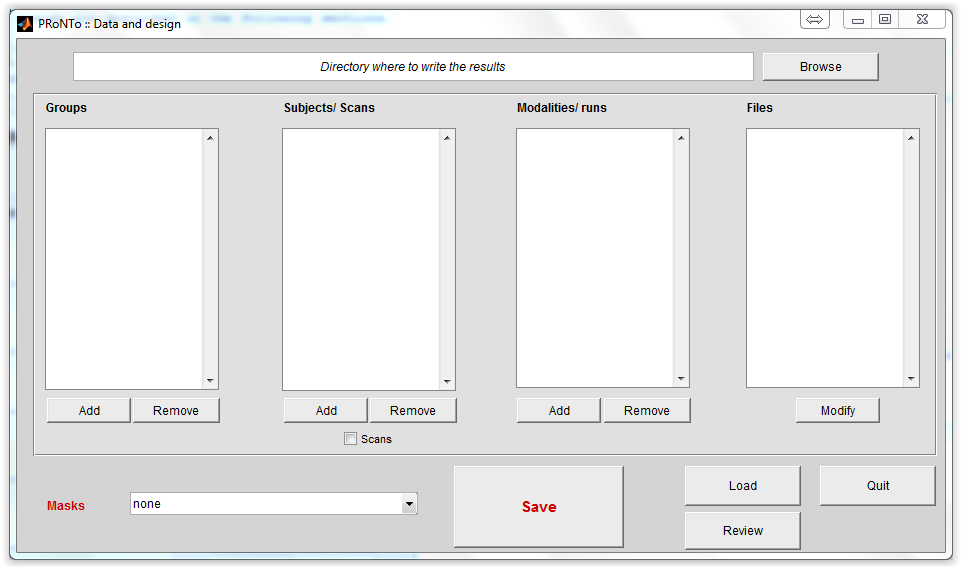
\includegraphics[height=2.7in]{images/Figure2.png}
   \caption{Data and design graphical user interface. This interface allows the user to enter all the information relative to the data, including the experimental design and masks. After introducing all the fields, PRoNTo creates the PRT structure, which is saved in the specified directory, as `PRT.mat' file.}
    \label{Fig2.2}
  \end{center}
\end{figure}

\subsection{PRT directory}

The first thing the user should specify is the directory in which to save the PRT structure. This can be done by browsing existing directories (previously created by the user) from the top of the data and design interface (Figure \ref{Fig2.2}). It is recommended to have different directories for different datasets (note that a dataset can include different modalities in case of multimodal analysis) because PRoNTo overwrites an existing PRT in the selected directory. The later modules in PRoNTo will then add more fields to this structure with further information, such as the models, features and kernels used in subsequent analyses. The file created is called `PRT.mat'.

\subsection{Groups}

The group panel allows one to add or remove a group of subjects. The minimum number of groups is one, but there is no maximum number. When `Add' is clicked, the user should provide a name to the group. Any alphanumeric string is sufficient and there should be no spaces in the string (this applies to all names throughout the toolbox). The name of the group can be later modified by right clicking on the name. When `Remove' is clicked, all the information relative to this group (including all subjects and corresponding data) is deleted. PRoNTo does not restore the deleted information and it can only be re-entered again by clicking `Add'.

The following panel after `Groups' is `Subjects/Scans'. Here, as mentioned above, there are two ways of entering the data: by `subjects' or by `scans'. The former is chosen by clicking `Add' under the `Subjects/Scans' panel and filling in the fields for each added subject at a time. The latter is done by clicking the tick box `Scans' under the `Subjects/Scans' panel. The subjects panel is then de-activated and the user can enter the modalities and files straight away. The fields to be filled under these two options are described below.

\subsection{Subjects}

\paragraph{Select by scans} The `select by scans' option allows the users to skip the subject step. To identify that this option has been selected, PRoNTo writes `scans' in the subjects panel (Figure \ref{Fig2.3}). The user can then add modalities and for each modality a new window will appear (bottom of Figure \ref{Fig2.3}). 

%It is important to remember that when the `scans' box is clicked all the information in the subjects panel is automatically deleted! 
% NOTE:AR-edit, no need for so many exclamations
It is important to remember that when the `scans' box is clicked all the information in the subjects panel is
automatically deleted. 
Unselecting the `scans' box also deletes all the information!

\paragraph{Select by subjects} The `Subjects/Scans' panel allows the user to add/remove subjects. This panel works exactly like the groups panel, but the subject name is automatically generated. This name can be later modified by right clicking on it. For each subject one can then specify the modalities in the next panel.

\begin{figure}[!h]
  \begin{center}
      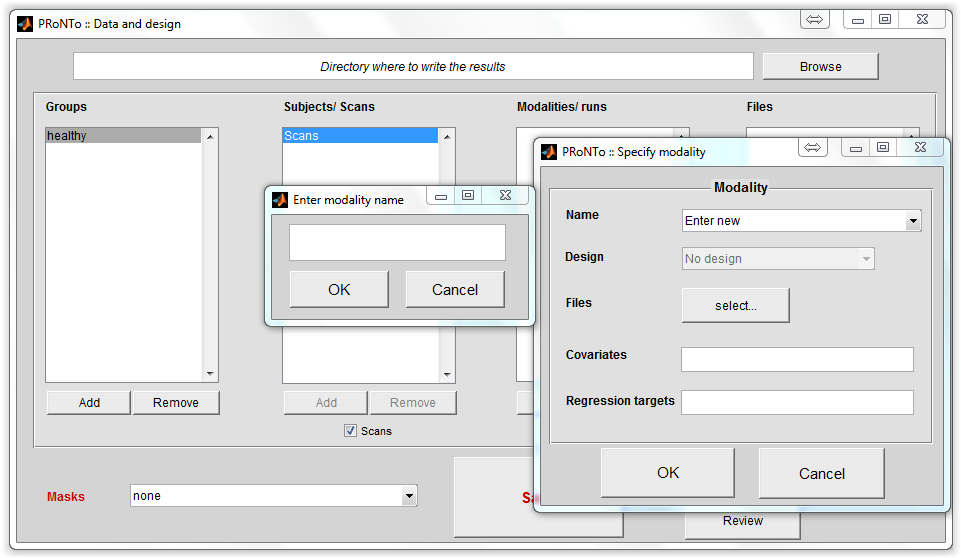
\includegraphics[height=3.5in]{images/Figure3.png}
   \caption{Data and design graphical user interface. If one chooses to specify everything using the `Scans' option (tick box below the `Subjects/Scans' panel), one can introduce the data for all subjects at once for each modality, but one cannot specify any design. This is the optimal approach when one has a lot of subjects with only one image/scan per subject, such can be the case of MRI and PET datasets.}
    \label{Fig2.3}
  \end{center}
\end{figure}

\subsection{Modalities} 

The modalities panel works like the group and subjects panel, but allows one to add and remove modalities. When a modality is added, a name needs to be provided (unless the modality has already been defined for a previous subject or through the masks menu, see below). It is important to note that a different modality can be a different type of data, such as fMRI and PET, or a different session of the same type of data, e.g. different runs/sessions of the same fMRI experiment. This way the different sessions can be integrated later into the same model and analysis.

The steps to enter the modality information are slightly different if one ticks the `scans' box or not.

\paragraph{Select by scans} Here the data is assumed to have been acquired without an experimental design, and therefore the `No design' option is automatically selected and cannot be changed (bottom window in Figure \ref{Fig2.3}). However, in select by scans, the user can also introduce `Covariates', i.e. a variable that covaries with the data (subjects) but of no interest to the subsequent analyses. This option will be functional in version 2.1 of PRoNTo. It requires the input of a matrix, with one row per image/subject. This matrix can either be entered as a Matlab command in the editable box, or the full path to a .mat containing the matrix should be provided (matrix named  `R'). This last option is recommended to input a matrix (i.e. more than one covariate). The last empty field can be used to enter `Regression targets'  (Figure \ref{Fig2.3}). This option allows the users to introduce a real number per subject to be used later for regression if that is the case. 
%As mentioned above, this is the only way of entering the data and regression values when doing \textit{Regression} models!
% NOTE:AR edit
As mentioned above, this is the only way of entering the data and regression values when doing
\textit{Regression} models.
\paragraph{Select by subjects} When entering the data by subjects, the modality window allows one to specify the experimental design (Figure \ref{Fig2.3}). Here there are three options. The last option is simply `No design', which means that for this modality there are no experimental conditions (this option is normally used when there is only one image per subject e.g. structural MRI or beta images from GLM analysis). The first option is to load an SPM.mat with a previously specified design. This option can be chosen if the user has created an SPM structure containing all the experimental fields using the SPM software. In this case, the user does not need to specify anything else, only the files (scans/images) for this subject/modality. The design information is extracted directly from the SPM structure and saved in PRT.mat. Finally, the `Specify design' option allows one to introduce all the conditions (durations and onsets), TR and other parameters corresponding to the experimental paradigm used for this subject and modality (this option is normally used with time series data, e.g. fMRI). After the design of the first subject has been specified, a new option will appear in the menu that allows to `Replicate design of subject 1', for the same modality and group. This facilitates design specification for groups of subjects with controlled (i.e. non-random) event onset and duration.

\begin{figure}[!h]
  \begin{center}
      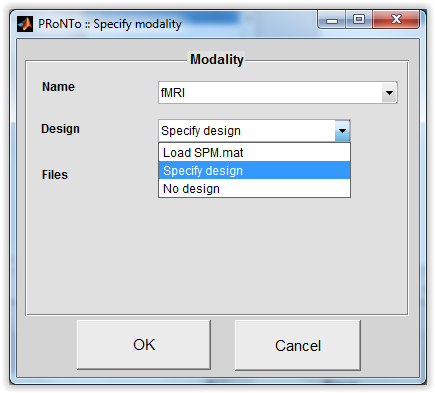
\includegraphics[height=3in]{images/Figure4.png}
   \caption{Data and design graphical user interface. The design menu in the modality window (when one uses the select by subject option) allows one to load a previously specified design from an SPM.mat file, create a new design or simply select no design, which usually applies to modalities where there is no experimental task, such as MRI or PET.}
    \label{Fig2.4}
  \end{center}
\end{figure}

\paragraph{Design} To create a new design one selects the option `Specify design' as explained in the previous paragraph (Figure \ref{Fig2.4}). This will then open another window (after choosing how many conditions you have) (Figure \ref{Fig2.5}). In this window one can then write the names, onsets, and durations of each condition. The units in which this information is read is specified below. There are two options `Scans' or `Seconds'. If the unit scans is selected, it is good to bear in mind that PRoNTo follows the convention, adopted in SPM, that the first scan is scan 0. In the durations field, one can introduce as many values as the number of onsets or just simply one value, which assumes the events all have the same duration. In this window there is also the option of introducing the Interscan Interval (TR), which is always read in seconds. 

One issue to have in mind when specifying the design is the following: if there are more scans than experimental events, these extra scans will not be used in later analyses. They are not deleted and the corresponding indexes can be found in the PRT structure: \\ PRT.group(g).subject(s).modality(m).design.conds(c).discardedscans. 

\begin{figure}[!h]
  \begin{center}
      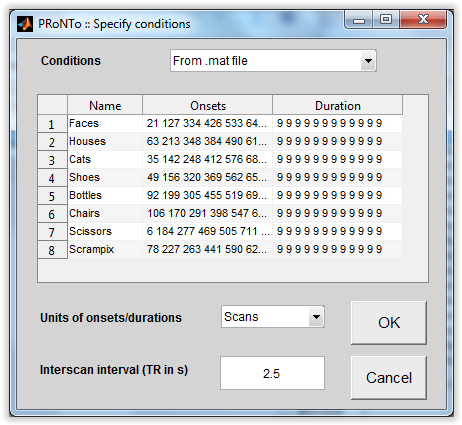
\includegraphics[height=3.5in]{images/Figure5.png}
   \caption{Data and design graphical user interface. The `specify conditions' window is available from the modality interface when the user chooses to enter the data by subjects and clicks `specify design'. This window is used to enter the conditions (names, onsets and durations) as well as the units of design, TR and covariates. }
    \label{Fig2.5}
  \end{center}
\end{figure}


\paragraph{Modify design}

The user can later modify a design by loading a PRT.mat in the Data and Design window. Please note that if feature sets or models have been previously computed, they will be discarded if changes are performed to the dataset. If the user wants to keep those, he/she should change the directory before saving any modification to the design. 

After loading a previously saved PRT, any change can be performed: subjects, groups or files can be added or removed. If the design needs to be modified, a right-click (ctrl+left-click in Mac) on the name of the concerned modality proposes to re-open the modality definition window. To review or modify the onsets/durations/blocks, the user can access their definition via the `specify design option'. Similar right-clicks (ctrl+left-click in Mac) allow renaming groups or subjects.

To modify the HRF parameters (delay or overlap), there is no need to load the PRT in Data and Design. Loading it within the Data Review allows the user to keep all previously computed feature sets and models. However, if the HRF parameters are changed, feature sets have to be computed anew since they do not correspond to the modified design. Changing the desired parameter (e.g. replacing `0' by `6') and hitting the `return' key updates the PRT directly in terms of scans selected for modelling. 
Please remember to keep an eye on the Matlab window, since important information are displayed on the workspace!

\paragraph{Files} Finally, independent of the way the user entered the information (by subjects or scans) the `Files' option allows one to choose which image files to use (Figure \ref{Fig2.6}). This will open another window that shows all image files available in each directory. These can be selected one by one or all at once, by using the mouse's right button on the right panel of the window (or shift key).

\begin{figure}[!h]
  \begin{center}
      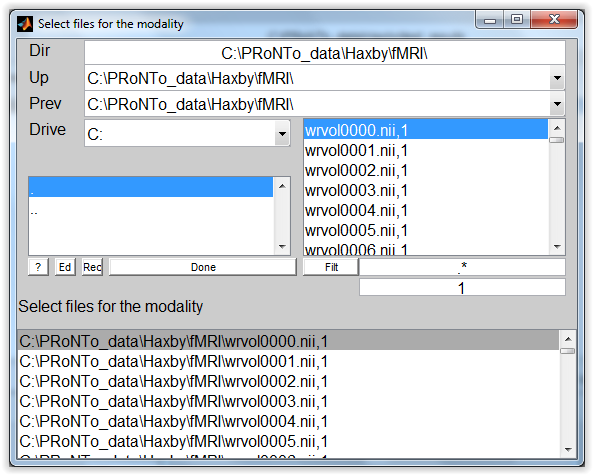
\includegraphics[height=3.2in]{images/Figure6.png}
   \caption{This window is called when one clicks `Files' and is used to select the scans/images for each subject/modality.}
    \label{Fig2.6}
  \end{center}
\end{figure}

All that is needed for each group, subject and modality has been specified and can now be viewed on the main window (Figure \ref{Fig2.7}) under each panel. The last panel shows which files have been entered for each modality and can be modified directly (click Modify). When Modify is clicked and no files are then selected all the previous files are deleted! Figure \ref{Fig2.7} shows how the data and design interface should look like once all the fields have been specified (using select by subject).
The design and files for each modality can also be modified by right clicking on the modality name in the modality panel. This option can be useful to visualise the design (onsets and durations) that has been previously entered and change it if necessary. For instance, one can check the design of the first subject and if changes are needed these can then be replicated for all other subjects as explained above.

\begin{figure}[!h]
  \begin{center}
      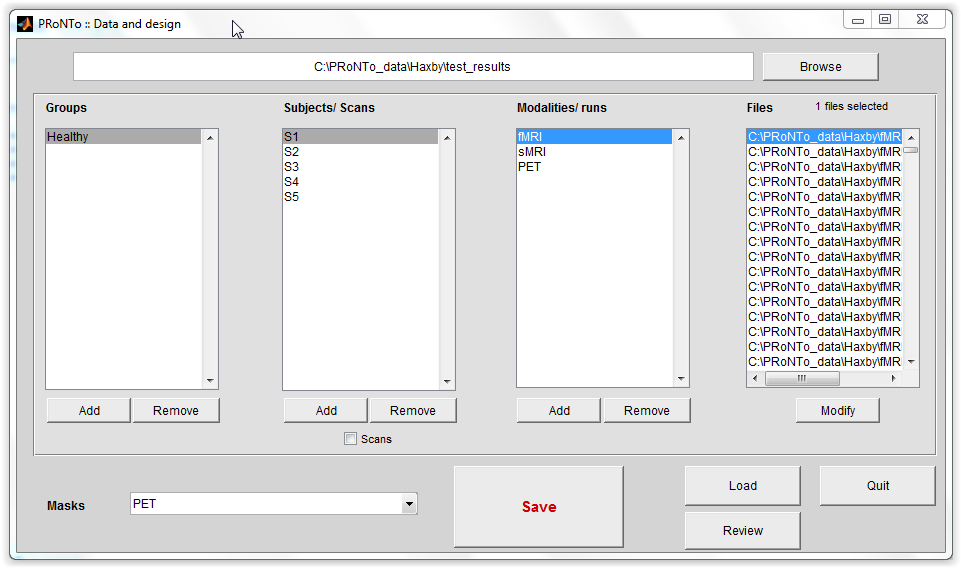
\includegraphics[height=2.85in]{images/Figure7.png}
   \caption{Data and design graphical user interface. After filling in all the fields using the select by subject option (the select by scans case is very similar) the data and design interface should look like this example figure.}
    \label{Fig2.7}
  \end{center}
\end{figure}


\subsection{Masks}

This popdown menu on the bottom of the main data and design window is where the user enters a binary image mask for each modality. This mask can be previously created by the user or simply chosen from a list of default masks available in the masks directory of PRoNTo. Every modality has to have a mask, which can be the same for all modalities. This is a first-level mask and is used simply to optimise the prepare feature set step by discarding all uninteresting features, such as voxels outside the brain. Later in the analysis one can choose another mask (second-level mask) that is more relevant to the scientific question and that can, for example, restrict the analysis to certain areas of the brain. To specify the mask one needs only to select the modality and then enter an image file. If the modalities have not yet been created, then one can create the modalities here, which will then appear in the modality panel.

\textbf{Important note}: If the first-level mask overlaps with areas that do not have values (e.g. either 0 or NaN) in the specified images, those areas will still be taken into account for further analysis. This might affect the results if those areas are not the same across images (typically, performance will be lower). We therefore advise the user to check the overlap between the first-level mask and his/her data. In most cases, this will not be needed, but for the acquisition of e.g. specific slices, this is recommended. We provide a script to update the mask automatically for beta images derived from a SPM GLM analysis (see \ref{chap:intro}, Inputs and preprocessing).

\subsection{Review}

The `Review' button allows one to review the data and design for each modality (Figure \ref{Fig2.8}). On the top right is the information relative to the number of groups and modalities that have been entered. The plot on the left displays the number of subjects per group. This is particularly important to check if the design is too unbalanced in terms of subjects. Then on the bottom right panel is the design information for each modality (if the selected modalities have an experimental design). Here, the user can view the number of conditions and can also edit the parameters that control the HRF delay and overlap (as explained above). The user can change the default value of 0 seconds and the effect is immediately seen on the number of scans plotted on the left (number of selected scans and number of discarded scans for each condition). The higher the value of the HRF peak and overlap, the higher the number of discarded scans. One can also read on the main Matlab window information regarding which group/subjects have had some scans discarded. The information below the HRF parameters corresponds to the interval between successive scans before and after the HRF delay/overlap correction. These values also change according to the changes entered in the boxes above. Please note, as mentioned in the section `Modify design', that information regarding the PRT being updated after changing the HRF parameters is written on the main Matlab window. 
%Again if you have previously computed feature sets and models, you have to recompute them because they do not correspond to the data anymore (changing the HRF delay and overlap parameters changes the data). 
% NOTE:AR-edit
Once again, if you have previously computed feature sets and models, you have to recompute them because they do not correspond to the data anymore (changing the HRF delay and overlap parameters changes the data). 
The information regarding which scans have been removed or not from the analysis can be found in the PRT structure: \\
{\tt PRT.group(g).subject(s).modality(m).design.conds(c).hrfdiscardedscans}.

\begin{figure}[!h]
  \begin{center}
      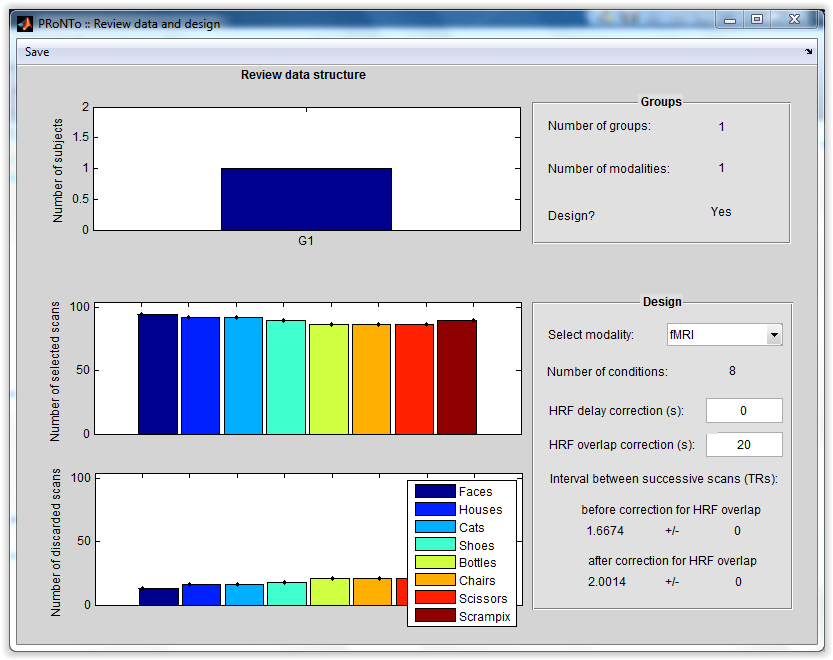
\includegraphics[height=4in]{images/Figure8.png}
   \caption{Data and design graphical user interface - `Review' window. This window allows the user to check the data and design, including the number of subjects per group. It also allows the user to change the HRF delay and overlap parameters that control the number of discarded scans (appropriate only for modalities such as fMRI). When there is no experimental design only the top plot and information is shown.}
    \label{Fig2.8}
  \end{center}
\end{figure}

\subsection{Load, Save and Quit}

The `Save' button allows the user to create the {\tt PRT.mat} file with the PRT structure containing all the information that has been specified here (Figure \ref{Fig2.7}). Incomplete information cannot be saved. At least one group should have all the required fields so that {\tt PRT.mat} can be created. `Load' allows the user to load the data and design information from a previously saved PRT.mat. The user can then edit the fields and update PRT by clicking again the `Save' button. It's very important to click `Save' because all the other steps in the analysis rely on the PRT structure. Without this structure one cannot proceed. However, when the {\tt PRT.mat} contains fields that have been added by the `Prepare feature set' or other modules, if the Save button is clicked, these fields will be deleted. The option `Quit' allows the user to leave the interface without saving the information. This is also the case when the user closes the window without first using the Save button.

\section{{\tt matlabbatch} interface}

The `Data and Design' module in the {\tt matlabbatch} is called either by first typing `prt' and clicking the `Batch' button or by typing `prt$\_$batch'. The user can then find on top of the batch a PRoNTo menu and under this menu the first module corresponds to the data and design module.

The options presented in the `Data and Design' GUI, mentioned above, are all available in the {\tt matlabbatch} interface (Figure \ref{Fig2.9}). However, there are a few things in the batch that differ from the GUI. One issue to note here is that, when using the batch one needs to be very careful with the names of the modalities specified for each subject (or using select by scans) and specified for each mask. The number of modalities should be exactly the same for each group and subject and the names should be consistent between groups/subjects and correspond to the names of the modalities under the masks field. In the GUI the names are made automatically consistent. The names of the conditions should also be the same across subjects and will be later used to define classes in the `Specify model' batch module.

Another issue is the HRF delay and overlap correction values. In the batch, the user can directly alter these values (instead of having to use the `Review' window) but the default is 0 seconds and should be changed (e.g. to 6 seconds) for modalities that depend on the HRF, such as fMRI.

As mentioned in the Introduction, the batch job can be saved as a .mat, and loaded again whenever needed, or as a .m that can be edited using the Matlab editor. This is a powerful tool that can make the specification of the data and design a lot easier and quicker, for example by editing and scripting existing batch files (for further information see the {\tt matlabbatch} chapter below).

\begin{figure}[!h]
  \begin{center}
      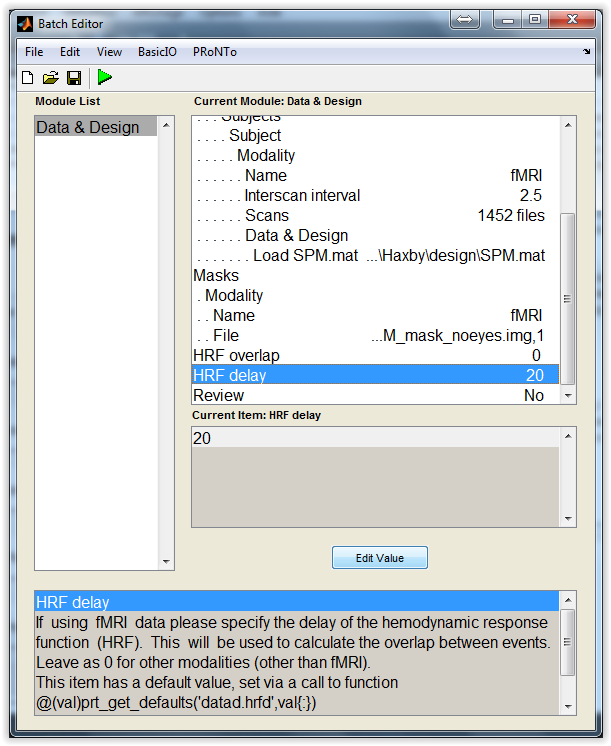
\includegraphics[height=4in]{images/Figure9.png}
   \caption{Data and design module in {\tt matlabbatch}. The {\tt matlabbatch} contains two extra options relative to the Data and Design interface. These options allow one to specify the delay and overlap of the HRF response (in the GUI it can only be changed in the `Review' window), and which are then used to determine the number of discard scans.}
    \label{Fig2.9}
  \end{center}
\end{figure}
